\section{Обзор предметной области и существующих решений}
\subsection{ClickHouse} \label{lit:ch}
ClickHouse - колоночная аналитическая система управления базами данных с открытым исходным кодом (распространяется под лицензией \textit{Apache Licence 2.0}). Создан и долгое время развивался в компании \enquote{Яндекс}, на момент написания статьи поддерживается и разрабатывается компанией ClickHouse Inc. Большая часть кодовой базы написана на языке C++ современного стандарта, разработка ведется в публичном GitHub репозитории (TODO: ссылка на мастер). 

В простейшем случае взаимодействие с ClickHouse опирается на две программы: \textit{clickhouse-server} и \textit{clickhouse-client}. Первая отвечается за управление базами данных и взаимодействие с клиентом, вторая - реализует клиентский интерфейс взаимодействия с сервером.

ClickHouse использует собственный язык запросов (ClickHouseQL), совместимый с SQL (см. Раздел \ref{lit:sql}), позволяющий клиенту выразить требуемые манипуляции с базами данных. Исходя из специфики ClickHouse, его язык запросов имеет особенности, выходящие за рамки стандартов SQL. Примером подобного отличия является поддержка ключевого слова \mintinline{sql}{ SAMPLE }, позволяющего получить случайную выборку из таблицы (см. Листинг \ref{lit:ch_ex}).

\begin{code}
    \captionof{listing}{Пример специфичных ClickHouseQL запросов (на примере SAMPLE)}
    \label{lit:ch_ex}
    \begin{minted}[frame=single, fontsize=\footnotesize]{sql}
SELECT value FROM table SAMPLE 0.1; -- relevant size
SELECT value FROM table SAMPLE 100; -- absolute size
SELECT value FROM table SAMPLE 0.1 OFFSET 0.1; -- with offset
    \end{minted}
\end{code}

Система сборки ClickHouse основана на комбинации \textit{ninja} + \textit{CMake}, сторонний код расположен в основном репозитории в виде \textit{git} сабмодулей (упрощенно - ссылки на другие репозитории). 

\subsection{MySQL} \label{lit:mysql}
MySQL - реляционная система управления базами данных с открытым исходным кодом (распространяется под лицензией \textit{GNU General Public License}), одна из наиболее распространенных СУБД в своем роде. На момент написаная работы, MySQL разрабатывается компанией \enquote{Oracle} 

MySQL использует собственный диалект SQL (см. Раздел \ref{lit:sql}), почти не противоречащий стандарту (TODO: ссылка на отличия), но расширяющий его новыми средствами. Примером может послужить нестрандартный \textit{null-safe} (корректно работающий с \mintinline{sql}{ NULL }) оператор сравнения \textit{<=>} (см. Листинг \ref{lit:mysql_ex}).

\begin{code}
    \captionof{listing}{Пример нестандартных SQL запроса в MySQL (на примере оператора <=>)}
    \label{lit:mysql_ex}
    \begin{minted}[frame=single, fontsize=\footnotesize]{sql}
SELECT NULL = NULL; -- NULL (not safe)
SELECT NULL <=> NULL; -- true (safe)
SELECT 1 <=> NULL; -- false
SELECT 1 <=> 1; -- true
SELECT 1 <=> 0; -- false
    \end{minted}
\end{code}

Стоит упомянуть так же некоторые типы запросов, не соответсвующие стандарту SQL, но поддерживаемые как MySQL так и ClickHouse (см. Листинг \ref{lit:non_standard}).

\begin{code}
    \captionof{listing}{Нестандартные SQL запросы общие для ClickHouse и MySQL}
    \label{lit:non_standard}
    \begin{minted}[frame=single, fontsize=\footnotesize]{sql}
USE database_name; -- choose default database by name;
SHOW TABLES; -- show all tables of choosen database
DESCRIBE table_name; -- show structure of a table by name;
    \end{minted}
\end{code}


\subsection{Формальные языки}
Термином \textit{алфавит} будем обозначать любое конечное множество симоволов. Например, множество $\{0, 1\}$ представляет собой бинарный алфавит. Другими широко известными примерами алфавитов являются \textit{ASCII} и \textit{Unicode}. 

\textit{Строка} (\textit{предложение}) над заданным алфавитом - конечная последовательность символов (возможно, пустая), принадлежащих алфавиту. Пустую строку будем обозначать за $\epsilon$. Примеры строк над алфавитом $\{0, 1\}$: \enquote{$010$}, \enquote{$0$}, \enquote{$1$}, $\epsilon$.

\textit{Формальный язык} - множество строк над фиксированным алфавитом. Примеры языков над алфавитом $\{0, 1\}$: множество всех строк длины 32 (конечное можество) множество строк, состоящих только из символа \enquote{$1$} (счетное множество). Множества $\varnothing$ и $\{\epsilon\}$ так же являются корректными языками над алфавитом $\{0, 1\}$. Заметим, что формальный язык не может быть несчетным множеством (это следует из того, что его элементами могут быть только строки конечной длины).

\subsection{Форма Бэкуса-Наура. Дерево разбора} \label{lit:bnf}

Формальный язык можно определять различными способами, например:
\begin{enumerate}
    \item Перечислением множества строк, составляющих язык (для конечных языков)
    \item Регулярным выражением
    \item Формой Бэкуса-Наура
\end{enumerate}

\textit{Форма Бэкуса-Наура} (сокр. \textit{БНФ}) - способ описания формального языка через четыре компонента:
\begin{enumerate}
    \item Множество \textit{терминалов} - элементарных символов языка. Примеры терминалов: \mintinline{c++}{ if } в языке C++, \mintinline{sql}{ SELECT } в языке SQL.
    \item Множество \textit{нетерминалов}. \textit{Нетерминал} определяется как множество строк \textit{терминалов}, удовлетворяющих правилам, описаным в следующем пункте
    \item Множество \textit{продукций}. Продукция - упорядоченная пара из \textit{нетерминала}, назваемого \textit{заголовком продукции}, и последовательности из терминалов и/или нетерминалов, называемой \textit{телом продукции}. Назначение продукции - описать правила, согласно которым \textit{заголовок продукции} может быть выражен через \textit{тело продукции}. \textit{Уточнение}: один и тот же нетерминал может входить в сколь угодно много продукций как в качестсве заголовка, так и как часть тела продукции.
    \item Один из нетерминальных символов, выделенный как \textit{стартовый} или \textit{начальный}
\end{enumerate}

При записи формы Бэкуса-Наура принято описывать продукцию как \enquote{\textit{заголовок продукции} $\rightarrow$ \textit{тело продукции}}, а элементы тела продукции записывать через пробел (обычно пробельный символ \textbf{не} входит в список терминальных символов). Так же считать стартовым нетерминалом заголовок продукции, расположенной выше остальных (при последовательной записи продукций).

Продукции, заголовки которых совпадают, обычно записывают в сокращенной форме по следующему принципу (см. Листинг \ref{lit:prod}):

\begin{code}
    \captionof{listing}{Компактная запись продукций с совпадающими заголовками}
    \label{lit:prod}
    \begin{minted}[frame=single, fontsize=\footnotesize]{text}
digit -> 0
digit -> 1

// same, but compact
digit -> 0 | 1
    \end{minted}
\end{code}

Символ \enquote{|} можно интуитивно воспринимать как \enquote{ИЛИ}. В примере выше продукции 1 и 2 в сумме эквиваленты продукции 3.

Ниже представлен пример записи простого формального языка включающий в себя натуральные числа (вместе с числом 0) и арифметические выражения, использующие операции \enquote{+} и \enquote{-} (без скобок), в форме Бэкуса-Наура: 
\begin{enumerate}
    \item Множество терминалов: цифры от 0 до 9, символы \enquote{+} и \enquote{-}
    \item Множество нетерминалов: \mintinline{text}{ expr }, \mintinline{text}{ number }, \mintinline{text}{ digit }
    \item Множество продукций: см. Листинг \ref{lit:bnf_ex}
    \item Стартовый символ: \mintinline{text}{ expr }
\end{enumerate}

\begin{code}
    \captionof{listing}{Компактная запись продукций с совпадающими заголовками}
    \label{lit:bnf_ex}
    \begin{minted}[frame=single, fontsize=\footnotesize]{text}
expr -> number + expr | number - expr | number
number -> digit number | digit
digit -> 0 | 1 | 2 | 3 | 4 | 5 | 6 | 7 | 8 | 9
    \end{minted}
\end{code}

Стоит обратить внимание на первую продукцию: в ней терминал \mintinline{text}{ expr } выражается сам через себя, что полностью корректно, хотя может показаться неинтуитивным с первого взгляда. Подобного рода продукции позволяют определять нетерминалы рекурсивно.

\begin{figure}[ht]
\begin{center}
\scalebox{0.25}{
    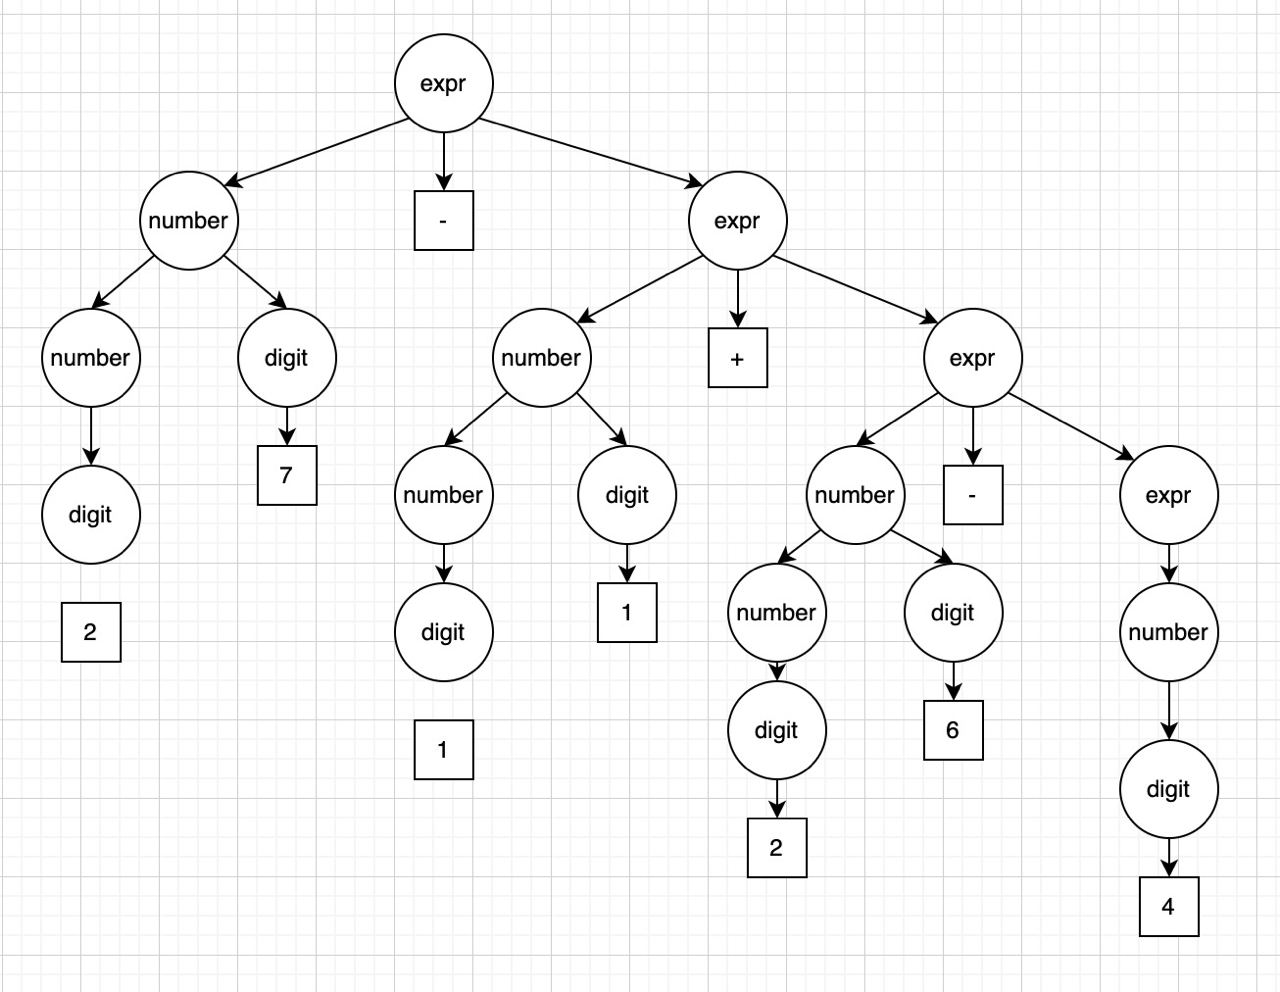
\includegraphics{images/bnf_ex_pic.jpg}
}
\caption{
\label{lit:bnf_ex_pic} Дерево разбора строки \enquote{27 - 11 + 26 - 4}
}
\end{center}
\end{figure}


Примеры строк, соотвествующих данному языку:
\begin{itemize}
    \item \mintinline{text}{ 2 + 2 }
    \item \mintinline{text}{ 27 - 11 + 26 - 4 }. Соответсвие этой строки данной форме Бэкуса-Наура проиллюстрировано ниже (см. Рис. \ref{lit:bnf_ex_pic}).
    \item \mintinline{text}{ 00012 } (определение нетерминала \mintinline{text}{ number } допускает ведущие нули)
\end{itemize}

Примеры строк, не соответсвующих данному языку:
\begin{itemize}
    \item \mintinline{text}{ abc + 1 } (символы \enquote{a}, \enquote{b}, \enquote{c} не входят в множество терминалов языка)
    \item \mintinline{text}{ 2 + 2 * 2 } (символ \enquote{*} не входит в множество терминалов языка)
    \item \mintinline{text}{ -1 } (не соответсвует ни одной из продукций из множества продукций языка)
\end{itemize}

Древовидная структура, отражающая соотвествие корректной строке правилам грамматики (в данном случае - форме Бэкуса-Наура), обозначается термином \textit{дерево разбора} или \textit{синтаксическое дерево}. Изображение ниже иллюстрирует пример дерева разбора (см. Рис. \ref{lit:bnf_ex_pic}). 

Будем называть языки, которые возможно задать через форму Бэкуса-Наура, \textit{контекстно-свободными языками}. \textit{Уточнение}: формально, класс контекстно-свободных языков может быть определен без использьзования БНФ через \textit{иерархию Хомского} (TODO ссылка), однако в рамках данной работы это не требуется.

Построение дерева разбора часто используется для того, чтобы в дальнейшем интерпретировать \textit{семантику} выражения на формальном языке (например, на языке программирования). На практике анализ предложения раздляют на два последовательных этапа: лексический и синтаксический анализ

\subsection{Лексический анализ}
Лексический анализ представляет собой процесс \textit{сканирования} последовательности символов исходного предложения (для простоты - последовательности байт) с целью:

\begin{itemize}
    \item Выделить значимые для языка фрагменты , называемые \textit{лексемами}
    \item Исключить из рассмотрения символы, не имеющие значения для языка (пробельные символы, комментарии, и т. д.)
\end{itemize}

\textit{Лексер} - программа, осуществляющая лексический анализ. Результатом работы лексера является последовательность \textit{токенов} - упорядоченной пары вида (тип токена, значение лексемы). Рассмотрим строку кода на C++ с точки зрения лексера (см. Листинг \ref{lit:lexer_ex_cpp}):

\begin{code}
\captionof{listing}{Строка кода на C++ с точки зрения лексера}
\label{lit:lexer_ex_cpp}
\begin{minted}[frame=single, fontsize=\footnotesize]{c++}
int foo = 1;
\end{minted}
\end{code}

Результатом работы лексера при анализе строки кода, приведенной выше может быть следующая последовательность токенов: (\textbf{var\_type}, int), (\textbf{identifer}, foo), (\textbf{assign\_op}, =), (\textbf{int\_literal}, 1), (\textbf{semicolon}, ;)

Полученная последовательность токенов используется в синтаксическом анализе в качестве входных данных. Все возможные типы токенов должны составлять \textit{терминалы формального языка}.

\subsection{Синтаксический анализ}
Задача синтаксического анализа в большинстве случаев - сконструировать дерева разбора, соотвествующее правилам грамматики (выраженной, например, при помощи БНФ), по последовательности токенов, полученной от лексера.

\textit{Парсер} - программа, осущесвтляющий синтаксический анализ. 

Можно заметить, что все действия, выполняемые лексером, можно осуществить и парсером. Однако,  использовние лексера позволяет абстрагировать парсер от излишней работы по распознавания символов. Модифицируем описаный ранее БНФ (см. конец Раздела \ref{lit:bnf}), полагая, что лексер распознает следующие токены (используя регулярные выражение):
\begin{itemize}
    \item \enquote{\mintinline{text}{[1-9][0-9]* }} - \mintinline{text}{ TOK_NUMBER } (десятичное число без ведущих нулей)
    \item \enquote{\mintinline{text}{\+ }} - \mintinline{text}{ TOK_PLUS_OP }
    \item \enquote{\mintinline{text}{- }} - \mintinline{text}{ TOK_MINUS_OP }
\end{itemize}

БНФ описывающий правила синтаксического анализа примет вид:
\begin{enumerate}
    \item Множество терминалов: \mintinline{text}{ TOK_NUMBER }, \mintinline{text}{ TOK_PLUS_OP }, \mintinline{text}{ TOK_MINUS_OP }
    \item Множество нетерминалов: \mintinline{text}{ expr }
    \item Множество продукций: см. Листинг \ref{lit:parser_bnf}
    \item Стартовый нетерминал: \mintinline{text}{ expr }
\end{enumerate}

\begin{code}
\captionof{listing}{БНФ парсера, использующий токены лексера}
\label{lit:parser_bnf}
\begin{minted}[frame=single, fontsize=\footnotesize]{text}
expr -> TOK_NUMBER + expr | TOK_NUMBER - expr | TOK_NUMBER
\end{minted}
\end{code}

\begin{figure}[ht]
\begin{center}
\scalebox{0.25}{
    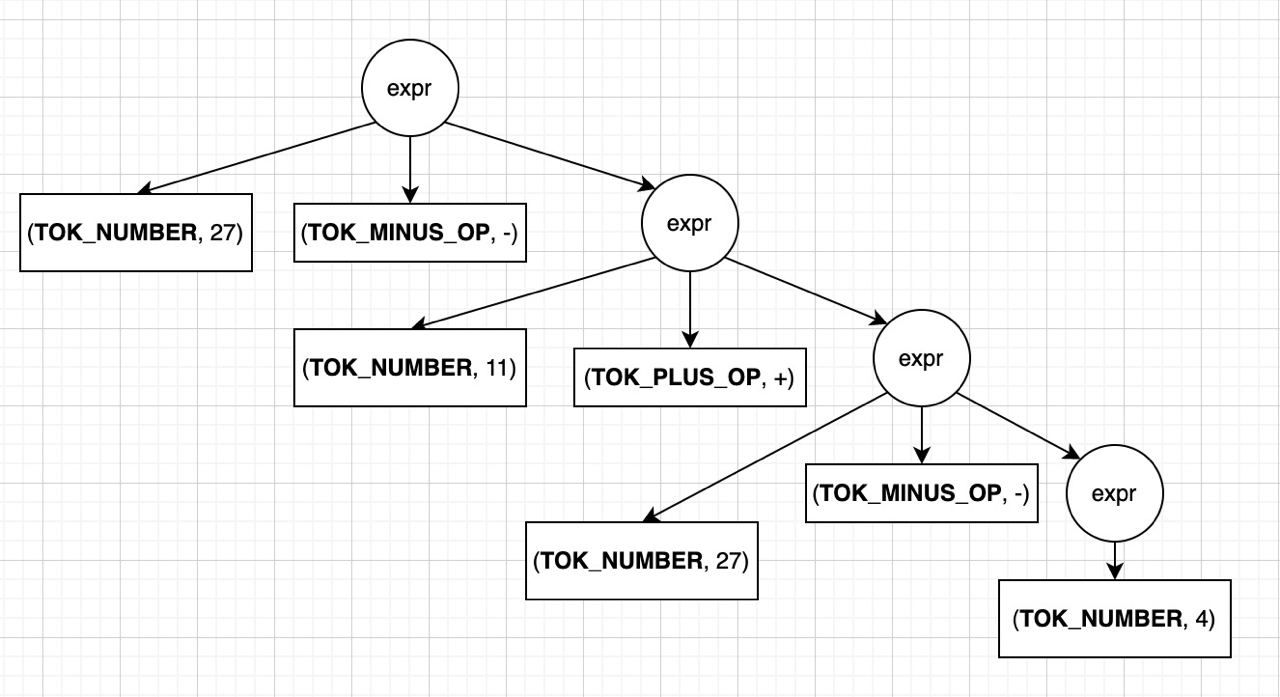
\includegraphics{images/parser_bnf_pic.jpg}
}
\caption{
\label{lit:bnf_ex_pic} Дерево разбора строки \enquote{27 - 11 + 26 - 4}, версия с лексером
}
\end{center}
\end{figure}

Можно отметить положительные результаты того, что лексический анализ был выделен в отдельную стадию: уменьшилось число продукций в БНФ, язык теперь не включает выражения с числами, содержащими ведущие нули. Дерево разбора, полученное в связке лексера и парсера (см. Рис. \ref{lit:parser_bnf_pic} так же отличается в лучшую сторону от дерева, полученного только с использованием парсера (см. Рис. \ref{lit:bnf_ex_pic})

\subsection{Абстрактное синтаксическое дерево}
TODO: ввести понятие абстрактного синтаксического дерева, аббревиатуру AST, сказать, что данная работа будет по большей части оперировать именно с AST

\subsection{ANTLR}
TODO: для поддержки MySQL диалекта в ClickHouse будет внедрен парсер MySQL использующий ANTLR для автоматической генерации исходного кода анализаторов. Объяснить что такое ANTLR и как устроена генерация (вкраце)


\subsection{SQL} \label{lit:sql}
SQL (сокр. от structured query language) - декларативный язык программирования, применяемый для выражения операций (создание, модификация, поиск и т. д.) над данными в базах данных (чаще всего - в реляционных). Как формальный язык, SQL является контекстно-независимым.

Ниже представлены примеры корректных выражений (строк, с точки зрения формального языка) на языке SQL:
\begin{code}
\captionof{listing}{Примеры выражений на языке SQL}
\label{lit:sql_ex}
\begin{minted}[frame=single, fontsize=\footnotesize]{sql}
SET str_param = 'str_value', int_param = 1; /* set parameters */
SELECT col1 FROM table WHERE col2 > 0; /* select data from table */
INSERT INTO table(col1, col2) VALUES (27, 27); /* insert new data into table */
UPDATE table SET col1 = 26 WHERE col2 = 27 /* modify existing row in table */
DROP TABLE table; /* delete existing table */
\end{minted}
\end{code}

Язык SQL является широко распространенным, общепринятым способом взаимодействия между СУБД и клиентом. Однако большинство СУБД не используют SQL в \enquote{чистом виде} (полностью в соответсвии со стандартом), а поддерживают собственные \textit{диалекты} SQL, например:
\begin{itemize}
    \item Диалект MySQL в реляционной CУБД MySQL (см. Раздел \ref{lit:mysql})
    \item ClickHouseQL в аналитической колоночной СУБД ClickHouse (см. Раздел \ref{lit:ch})
    \item SphinxQL в СУБД Sphinx, ориентированной на полнотекстовый поиск
\end{itemize}

Ниже (см. Листинг \ref{lit:sql_dialect}) приведены примеры нестандартных запросов на различных диалектах SQL, специфичных для используемой СУБД (поддерживается ей и только ей):

\begin{code}
\captionof{listing}{Примеры отличительных запросов на диалекте SQL}
\label{lit:sql_dialect}
\begin{minted}[frame=single, fontsize=\footnotesize]{sql}
/* ClickHouseQL: select columns by regexpr */ 
SELECT columns("[a-zA-Z]+") FROM table;

/* SphinxQL: full-text search query */
SELECT id, titile FROM table WHERE MATCH('@description foo | bar');

/* MySQL dialect: null-safe equals operator */
SELECT 1 <=> NULL;
\end{minted}
\end{code}

\subsection{Обзор существующих решений}
TODO: я не успею предметно разобраться в существующих решениях, поэтому рассказ о них я не стал выделять в отдельную главу. Отмечу, что практика поддержки стронних SQL диалектов встречается не так часто, но постепенно обретает все большее распространение. Привету примеры СУБД, в которых эта поддержка реализована (список)

\subsection{Список терминов}
Дать определения прочим терминам, не являющимся ключевыми в данной работе, но которые знать для того, чтобы понять работу
\begin{enumerate}
    \item Юнит-тесты - ...
    \item Функциональные тесты - ...
    \item Скрипт - ...
    \item Вычитать работу и добавить сюда термины
\end{enumerate}

TODO: расставить здесь и в дальнейшем по работе ссылки на источники (пока что они не добавлены)

\pagebreak
